% ===========================================================================
\chapter{\label{chap:ferramenta}O \ferramenta}

Este capítulo descreve o artefato avaliado. A Seção~\ref{sec:visao} apresenta a visão geral e a arquitetura. As Seções~\ref{sec:mod1} a~\ref{sec:mod3} detalham os três módulos, com a definição formal dos indicadores que as QPs avaliam. A Seção~\ref{sec:fluxo} descreve o fluxo de dados sob a ótica da privacidade, e a Seção~\ref{sec:parametros} reúne os parâmetros da versão avaliada, necessários à reprodução.

\section{\label{sec:visao}Visão geral e arquitetura}

O \ferramenta é uma aplicação \estr{web} com um único papel de usuário: o estudante. O estudante organiza seus PDFs por disciplina, inicia sessões de estudo sobre um ou mais PDFs e consulta um painel com o próprio histórico. A Figura~\ref{fig:arquitetura} resume a arquitetura e o caminho de cada tipo de dado.

\begin{figure}[htbp]
\centering
\begin{tikzpicture}[
  font=\footnotesize,
  caixa/.style={draw, rounded corners=2pt, align=center, minimum height=10mm, minimum width=24mm, inner sep=3pt, fill=white},
  zona/.style={draw, dashed, rounded corners=4pt, inner sep=6pt},
  seta/.style={-{Stealth[length=2mm]}, thick},
  rot/.style={font=\scriptsize, align=center, inner sep=1.5pt}
]
% ---- Navegador
\node[caixa] (cam) at (0,0) {Câmera};
\node[caixa] (fm) at (3.6,0) {Detecção facial\\(MediaPipe)};
\node[caixa] (yolo) at (3.6,-1.6) {Detecção de celular\\(YOLOv8n, WASM)};
\node[caixa] (ind) at (7.4,-0.8) {\fs e\\eventos de celular};
\node[caixa] (ui) at (11.2,-0.8) {Interface (SPA)\\leitura, questões,\\painel};
\draw[seta] (cam) -- (fm);
\draw[seta] (cam.south) |- (yolo.west);
\draw[seta] (fm.east) -- ++(0.4,0) |- ([yshift=2mm]ind.west);
\draw[seta] (yolo.east) -- ++(0.4,0) |- ([yshift=-2mm]ind.west);
\draw[seta] (ind) -- (ui);
\begin{scope}[on background layer]
\node[zona, fit=(cam)(fm)(yolo)(ind)(ui), label={[font=\small\bfseries]above:Navegador do estudante}] (nav) {};
\end{scope}
\node[rot, text=red!60!black, anchor=south west] at (5.4,-2.35) {\textit{nenhum quadro de vídeo sai desta zona}};

% ---- Servidor
\node[caixa] (ing) at (0.6,-4.6) {Ingestão de PDF\\extração, limpeza,\\fragmentação};
\node[caixa] (api) at (5.6,-4.6) {API REST\\(FastAPI)};
\node[caixa] (db) at (10.4,-4.6) {Banco relacional\\sessões, questões,\\respostas, telemetria};
\node[caixa] (vet) at (0.6,-6.6) {Banco vetorial\\(ChromaDB)};
\node[caixa] (ger) at (5.6,-6.6) {Geração de questões};
\draw[seta] (api) -- node[rot, above]{PDF} (ing);
\draw[seta] (ing) -- (vet);
\draw[seta] (vet) -- node[rot, above]{fragmentos} (ger);
\draw[seta] (ger) -- node[rot, right]{questões} (api);
\draw[seta, {Stealth[length=2mm]}-{Stealth[length=2mm]}] (api) -- (db);
\begin{scope}[on background layer]
\node[zona, fit=(ing)(api)(db)(vet)(ger), label={[font=\small\bfseries, anchor=north west]south west:Servidor da aplicação}] (srv) {};
\end{scope}

\node[caixa, minimum width=20mm] (llm) at (5.6,-9.0) {Provedor do LLM\\(terceiro)};
\draw[seta, {Stealth[length=2mm]}-{Stealth[length=2mm]}] (ger) -- node[rot, right, pos=0.55]{fragmento de texto $\downarrow$\quad questão em JSON $\uparrow$} (llm);

% ---- Tráfego cliente-servidor
\draw[seta, {Stealth[length=2mm]}-{Stealth[length=2mm]}] (ui.south) -- ++(0,-1.3) -| (api.north);
\node[rot, anchor=north west, align=left] at (5.9,-2.9) {$\downarrow$ PDFs, respostas, telemetria agregada (\fs, eventos, modo)\\$\uparrow$ questões, dados do painel};
\end{tikzpicture}
\caption{Arquitetura do \ferramenta. Toda a visão computacional ocorre na zona tracejada superior (navegador); o servidor recebe apenas os PDFs enviados pelo estudante, as respostas às questões e a telemetria agregada. O único dado que sai do servidor para um terceiro é o fragmento de texto enviado ao provedor do LLM. Fonte: elaborada pelo autor a partir do código do protótipo.}
\label{fig:arquitetura}
\end{figure}

A arquitetura segue uma regra simples: o que envolve a imagem do estudante fica no cliente; o que envolve o texto do material fica no servidor. O cliente é uma aplicação de página única (\estr{Single Page Application}, SPA) em Angular, que executa os dois modelos de visão computacional. O servidor, em Python com FastAPI, recebe os PDFs, mantém o banco vetorial e o banco relacional e orquestra as chamadas ao modelo de linguagem. A escolha do FastAPI se deve ao tratamento nativo de entrada e saída assíncrona e à validação declarativa dos dados recebidos, úteis para orquestrar chamadas a um serviço externo de latência variável e para garantir que a telemetria contenha apenas os campos esperados.

\section{\label{sec:mod1}Módulo 1: materiais e geração de questões}

\subsection{Ingestão do material}

O estudante cria uma disciplina e envia PDFs a ela (Figura~\ref{fig:materiais}). Cada PDF percorre quatro etapas. Primeiro, o texto é extraído página a página. Em seguida, uma etapa de limpeza remove hifenizações de fim de linha, junta linhas quebradas no meio de frases, normaliza marcadores de lista e descarta linhas repetidas, comuns em cabeçalhos e rodapés de apresentações. Depois, o texto limpo é fragmentado por um divisor recursivo que respeita, sempre que possível, quebras de parágrafo e de frase, com tamanho-alvo de 900 caracteres e sobreposição de 120 caracteres entre fragmentos consecutivos; fragmentos com menos de 80 caracteres são descartados. Por fim, os fragmentos são indexados no ChromaDB, em uma coleção por PDF.

\begin{figure}[htbp]
\centering
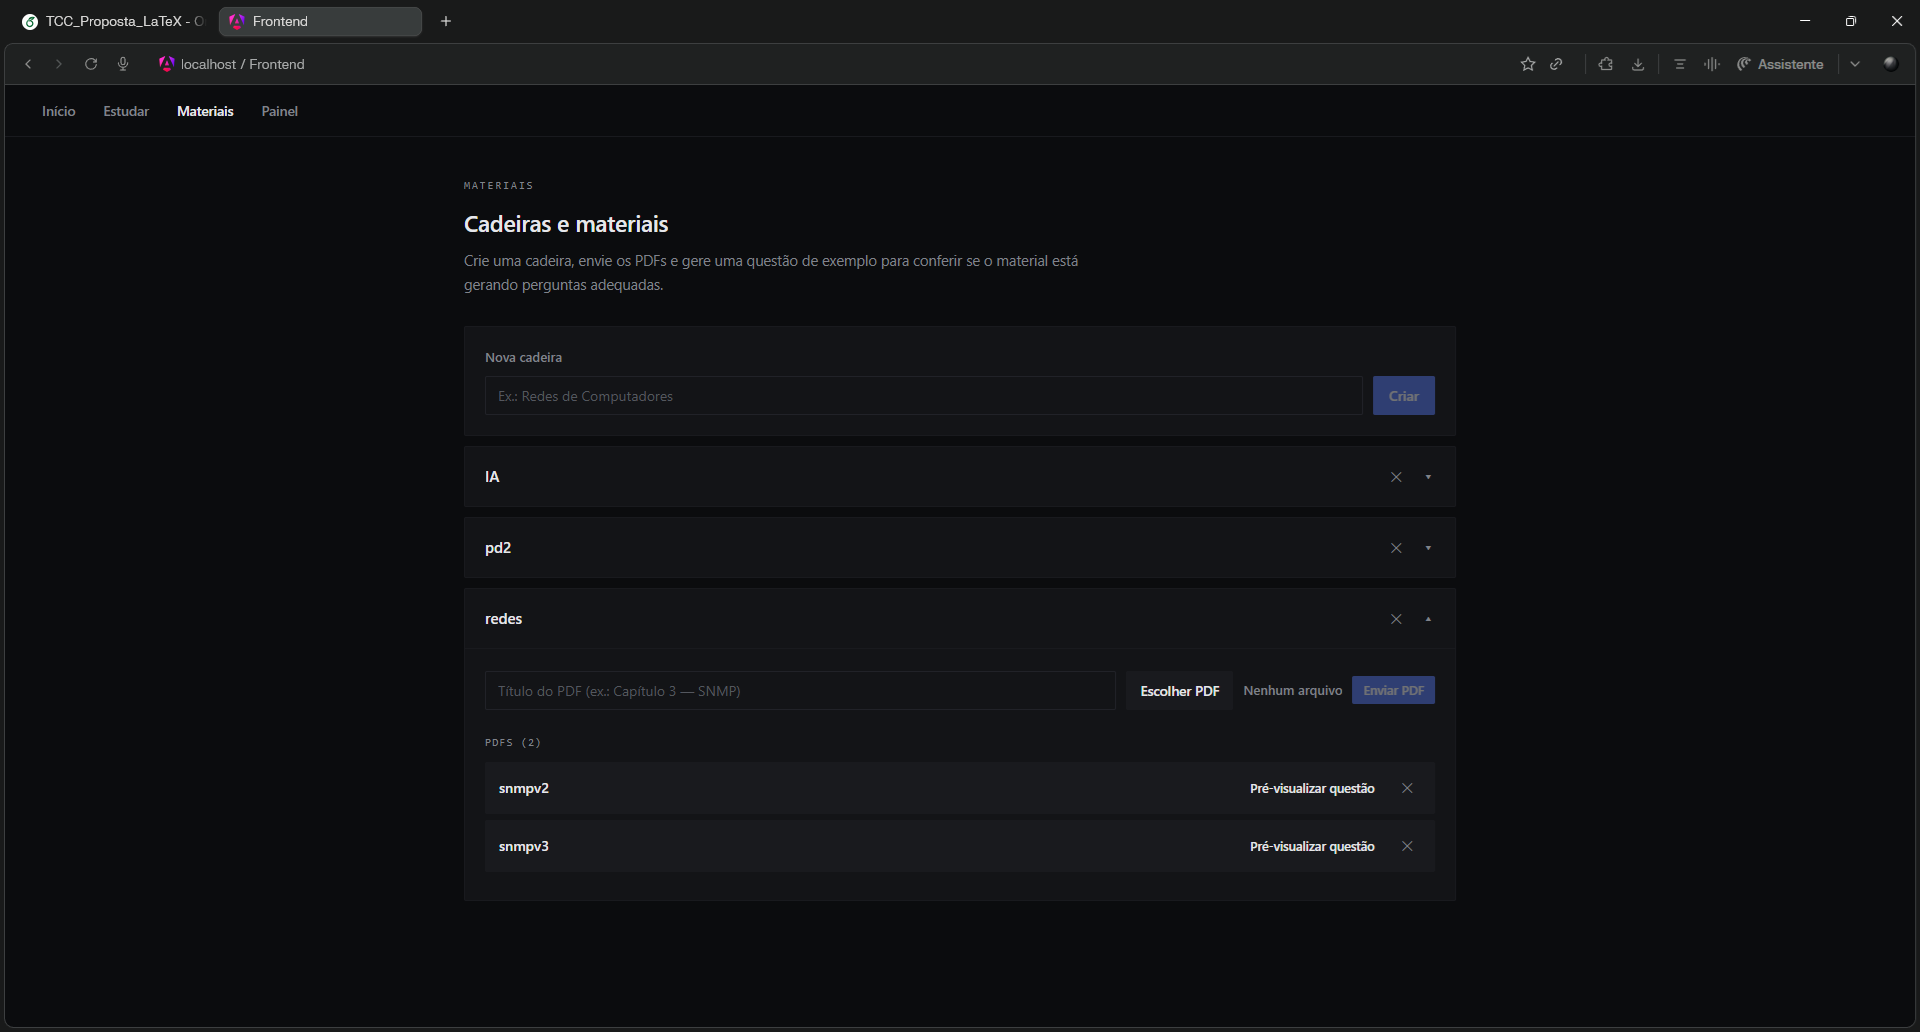
\includegraphics[width=0.85\textwidth]{materiais.png}
\caption[Tela de materiais do \ferramenta]{Tela de materiais: o estudante cria disciplinas, envia PDFs e pode pré-visualizar uma questão gerada a partir de um fragmento sorteado, para conferir se o material foi bem extraído. Fonte: captura do protótipo feita pelo autor. \definir{refazer a captura em tema claro, recortada e em resolução 2x}}
\label{fig:materiais}
\end{figure}

A sobreposição evita que uma ideia dividida entre dois fragmentos fique incompleta em ambos. O tamanho de 900 caracteres, aproximadamente dois parágrafos, busca um equilíbrio: fragmentos curtos demais não contêm informação suficiente para uma pergunta de compreensão, e fragmentos longos demais tornam difícil verificar se a resposta está neles. A sensibilidade dos resultados a esse parâmetro é avaliada na QP1 (Seção~\ref{sec:met-qp1}).

\subsection{Seleção do fragmento-fonte}

Nem todo fragmento de um PDF serve de base para uma pergunta: sumários, tabelas, listas de siglas e trechos de código produzem questões ruins. Antes da geração, cada fragmento passa por um filtro de utilidade que exige pelo menos 15 palavras e menos de 40\% delas em caixa alta, o que elimina a maior parte dos títulos e siglários. Se o filtro eliminar todos os fragmentos, o sistema usa os fragmentos originais, para não deixar o estudante sem questões. Dentre os fragmentos úteis dos PDFs selecionados para a sessão, o sistema sorteia os que servirão de fonte.

\subsection{Geração ancorada no fragmento}

Cada questão é gerada a partir de um único fragmento, chamado aqui de fragmento-fonte. O modelo recebe o fragmento e a instrução de criar uma questão de múltipla escolha em português, com enunciado respondível apenas com o conteúdo do trecho, quatro alternativas plausíveis e exatamente uma correta, acompanhada de uma justificativa. A resposta deve ser um objeto JSON com campos fixos. O prompt completo está no Apêndice~\ref{ap:prompts}.

Três cuidados complementam a geração. O primeiro é a validação do formato: respostas que não contêm um JSON válido ou que trazem menos de duas alternativas são rejeitadas. O segundo é o embaralhamento das alternativas após a geração, com a posição da correta recalculada, porque modelos de linguagem tendem a posicionar a alternativa correta de forma não uniforme. O terceiro é a rastreabilidade: o fragmento-fonte é gravado junto com a questão, o que permite, na revisão dos erros e na avaliação, conferir em que trecho a questão se baseou. Para reduzir a espera, as questões de uma sessão são geradas em lotes de cinco, em uma única chamada ao modelo, e o lote seguinte é solicitado enquanto o estudante responde ao atual.

Rigorosamente, o \ferramenta implementa uma variante da geração aumentada por recuperação. No RAG clássico, uma consulta do usuário é convertida em vetor e os fragmentos mais próximos são recuperados para compor o contexto. No \ferramenta, não há consulta: a ``recuperação'' é a escolha do fragmento que será perguntado, e o banco vetorial também permite recuperar os fragmentos vizinhos, semanticamente próximos, como contexto adicional. A versão principal gera a partir do fragmento-fonte isolado; a inclusão dos vizinhos é avaliada como ablação na QP1, justamente para medir se o contexto adicional melhora a questão ou a afasta do fragmento que deveria ancorá-la.

\section{\label{sec:mod2}Módulo 2: a sessão de estudo}

Ao iniciar uma sessão, o estudante escolhe os PDFs e uma de três atividades (Figura~\ref{fig:selecao}): responder a um questionário gerado do material; ler um material de estudo que o modelo produz a partir dos PDFs, adaptado ao nível, ao objetivo e ao tempo que o estudante declara; ou revisar as questões que errou em sessões anteriores. No questionário, cada resposta recebe \estr{feedback} imediato, com a indicação da alternativa correta e a justificativa (Figura~\ref{fig:quiz}), em linha com as condições de eficácia do \estr{feedback} discutidas na Seção~\ref{sec:perguntas}. O material de estudo gerado é um recurso de apoio e não é objeto da avaliação deste trabalho.

\begin{figure}[htbp]
\centering
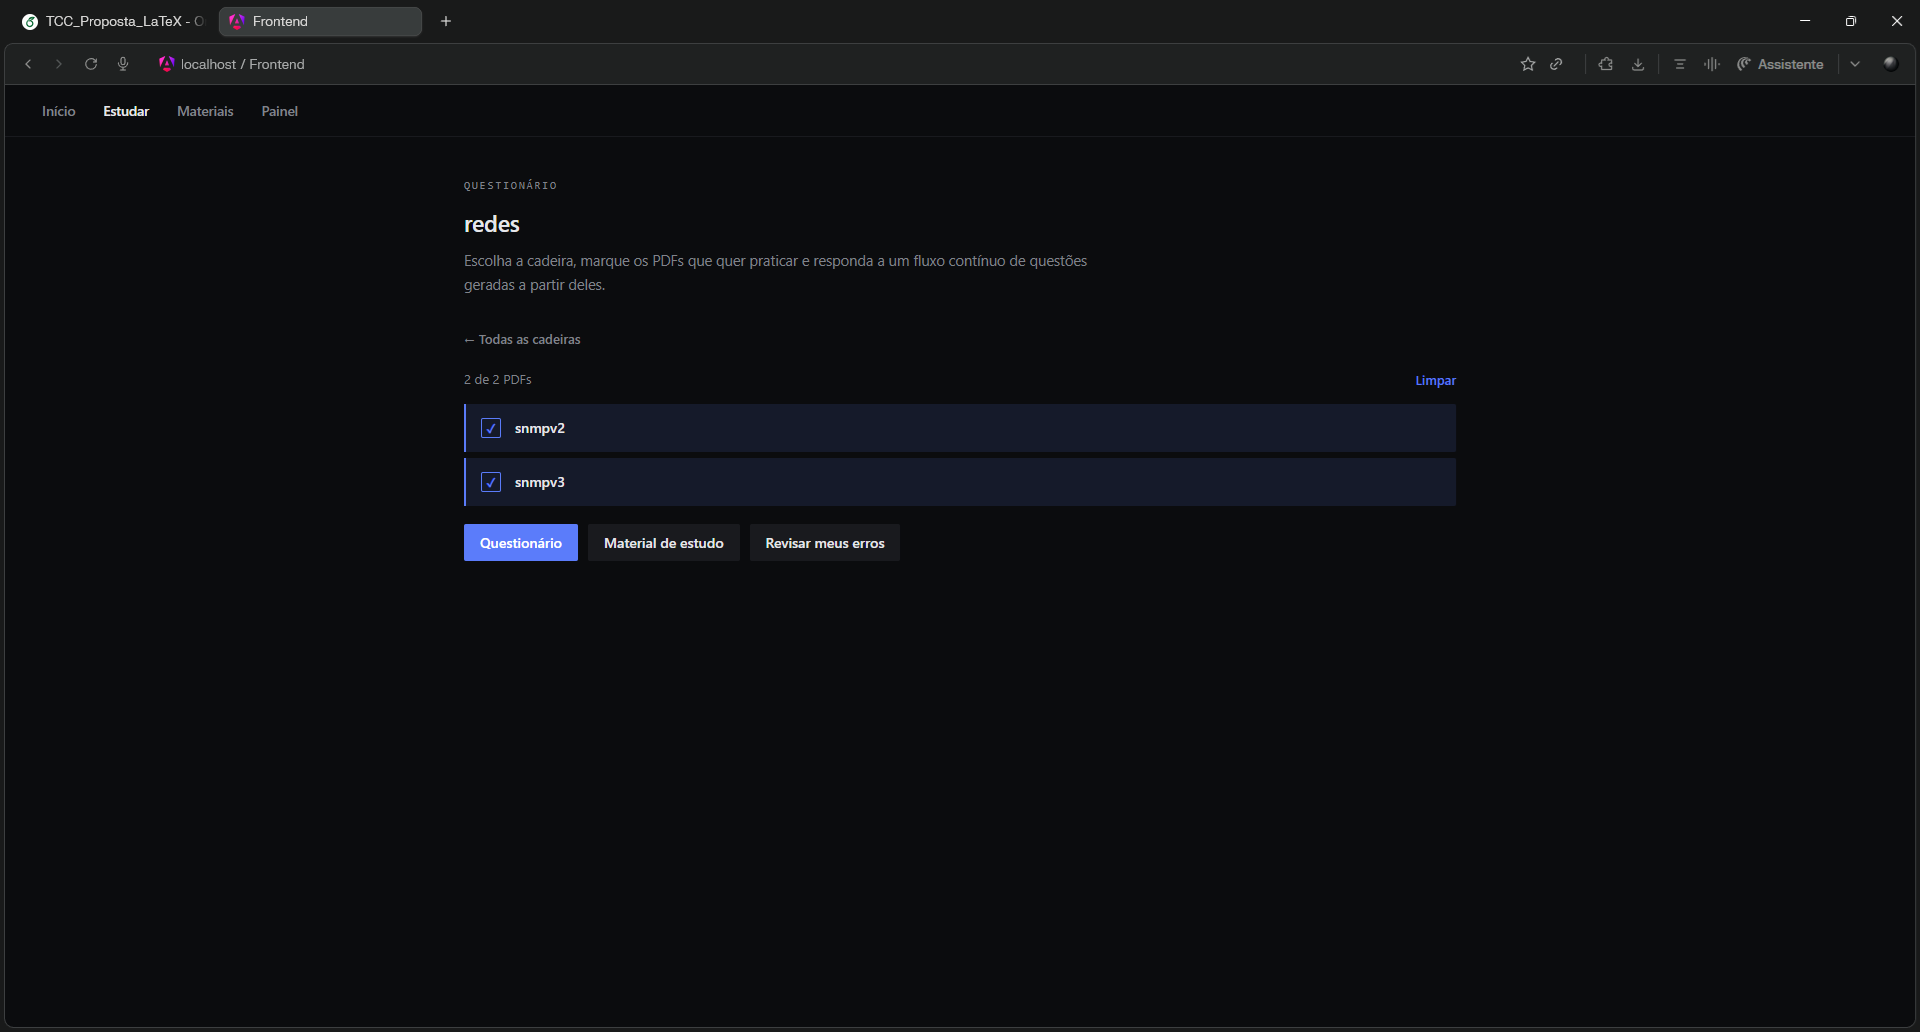
\includegraphics[width=0.85\textwidth]{selecao.png}
\caption{Início da sessão: seleção dos PDFs da disciplina e escolha entre questionário, material de estudo ou revisão dos erros. Fonte: captura do protótipo feita pelo autor.}
\label{fig:selecao}
\end{figure}

\begin{figure}[htbp]
\centering
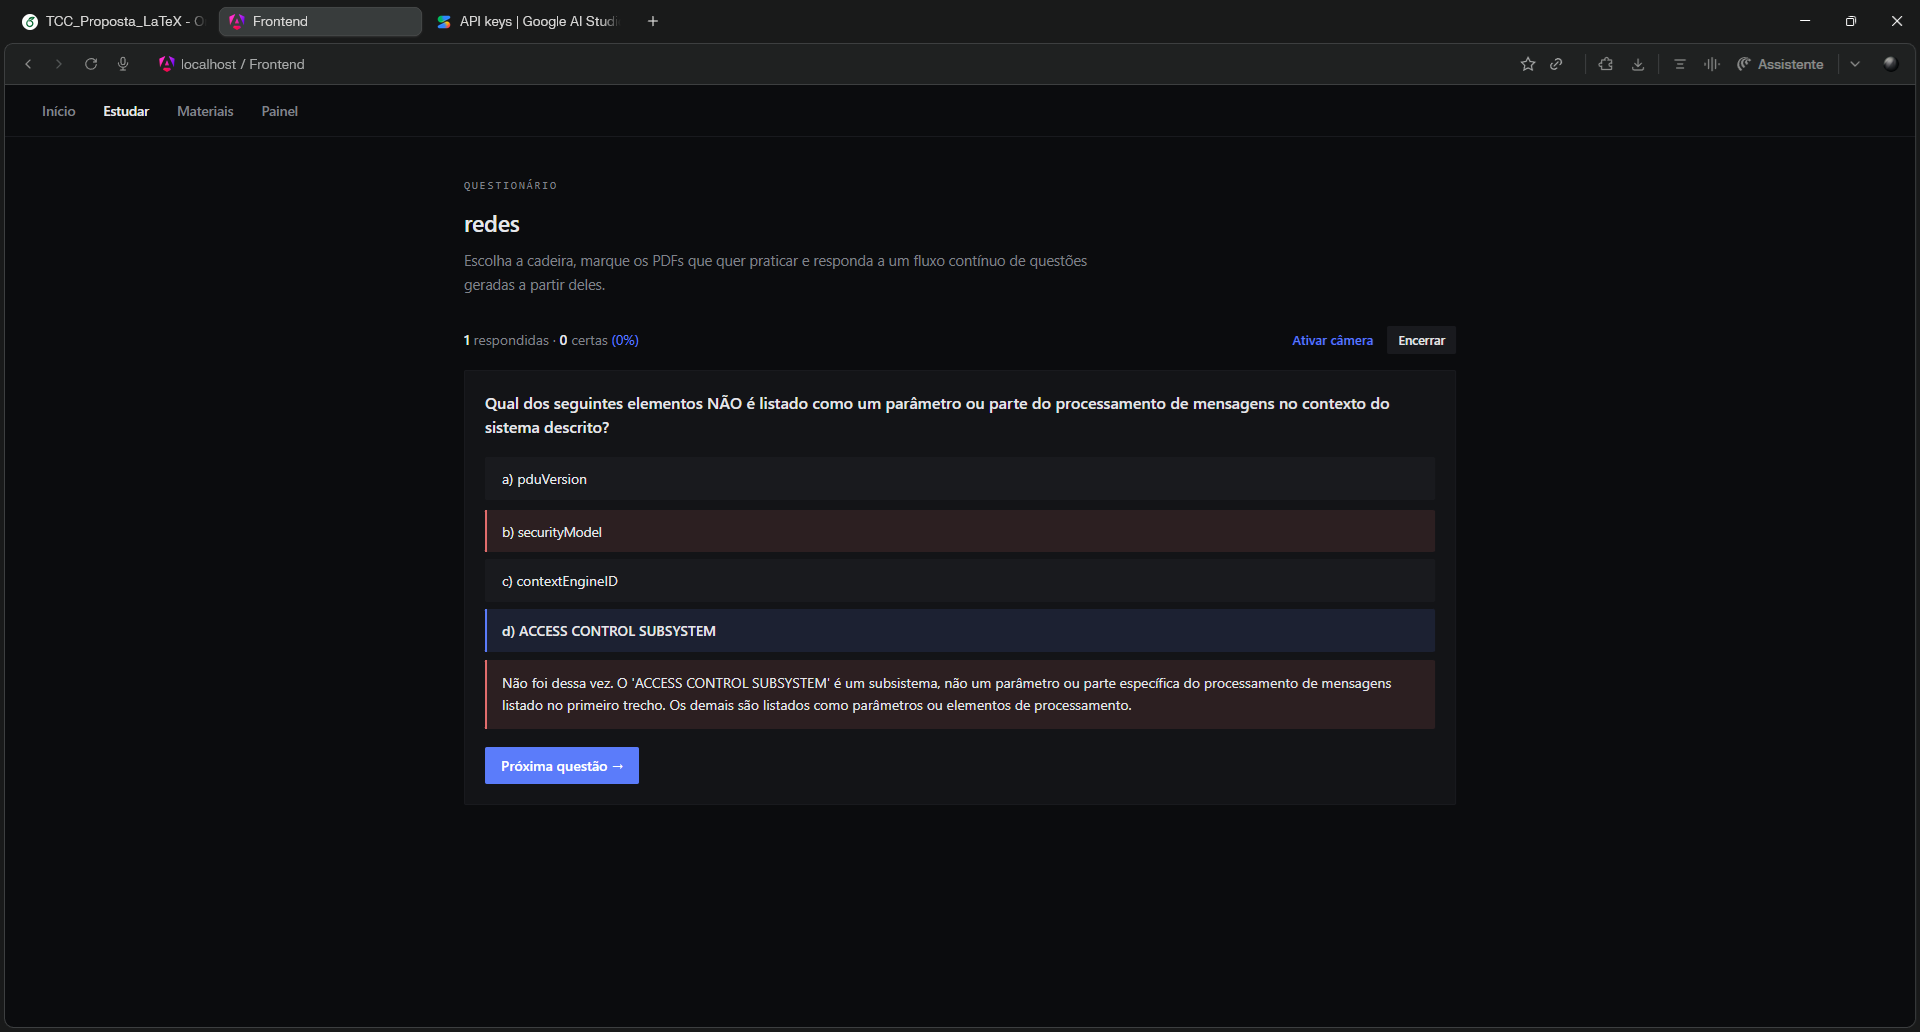
\includegraphics[width=0.85\textwidth]{quiz-feedback.png}
\caption{Questão gerada a partir de um fragmento do material, com \estr{feedback} imediato após a resposta: a alternativa correta é destacada e a justificativa é exibida. Fonte: captura do protótipo feita pelo autor.}
\label{fig:quiz}
\end{figure}

Com o consentimento do estudante, a câmera é ativada e dois processos passam a rodar no navegador: a estimativa do engajamento visual e a detecção de celular.

\subsection{\label{sec:focusscore}Engajamento visual: definição do \fs}

A cada quadro processado, o MediaPipe estima os pontos faciais a partir de um vídeo de 320$\times$240 \estr{pixels}. Três grandezas são calculadas sobre esses pontos.

A primeira é a EAR média dos dois olhos. Para cada olho, com os seis pontos $p_1,\dots,p_6$ dispostos ao seu redor ($p_1$ e $p_4$ nos cantos, $p_2,p_3$ na pálpebra superior e $p_6,p_5$ na inferior),
\begin{equation}
\mathrm{EAR} = \frac{\lVert p_2 - p_6\rVert + \lVert p_3 - p_5\rVert}{2\,\lVert p_1 - p_4\rVert}.
\label{eq:ear}
\end{equation}

A segunda e a terceira são aproximações da direção da cabeça, obtidas por razões entre coordenadas normalizadas dos pontos. A rotação horizontal (\estr{yaw}) é aproximada pela posição horizontal da ponta do nariz entre os dois contornos laterais do rosto, $y_{\mathrm{aw}} = (x_{\mathrm{nariz}} - x_{\mathrm{esq}})/(x_{\mathrm{dir}} - x_{\mathrm{esq}})$, que vale cerca de $0{,}5$ com o rosto de frente. A inclinação vertical (\estr{pitch}) é aproximada pela posição vertical da ponta do nariz entre a linha dos olhos e o queixo, $p_{\mathrm{itch}} = (y_{\mathrm{nariz}} - y_{\mathrm{olhos}})/(y_{\mathrm{queixo}} - y_{\mathrm{olhos}})$. Essas razões não são ângulos, mas variam de forma monotônica com eles e dispensam a estimativa de pose tridimensional.

Como os valores dessas grandezas variam entre pessoas, câmeras e posições, os primeiros cinco segundos da sessão são uma calibração, durante a qual o estudante olha para a tela. Ao final, o sistema guarda as medianas $\tilde{e}$, $\tilde{y}$ e $\tilde{p}$ da EAR, do \estr{yaw} e do \estr{pitch}, e define o limiar de olho aberto como $\theta = 0{,}72\,\tilde{e}$. O fator de $0{,}72$ foi ajustado em testes internos do autor e é objeto da análise de sensibilidade da QP3.

Após a calibração, cada quadro $i$ recebe um estado bruto $r_i \in \{0,1\}$, igual a 1 quando as três condições são satisfeitas simultaneamente:
\begin{equation}
r_i = \mathbb{1}\big[\text{rosto detectado}\big]\cdot
\mathbb{1}\big[\lvert y_{\mathrm{aw},i} - \tilde{y}\rvert < \tau_y \;\wedge\; \lvert p_{\mathrm{itch},i} - \tilde{p}\rvert < \tau_p\big]\cdot
\mathbb{1}\big[\mathrm{EAR}_i > \theta\big],
\label{eq:estado}
\end{equation}
com tolerâncias $\tau_y = 0{,}13$ e $\tau_p = 0{,}10$.

Um estado bruto igual a zero não significa necessariamente distração: piscar, olhar rapidamente para o teclado ou ajustar a postura produzem zeros de curta duração. Por isso, o sistema aplica um período de tolerância $g$: se o quadro $i$ pertence a uma sequência de estados brutos nulos iniciada no instante $t_d$, seu estado final é
\begin{equation}
s_i = \begin{cases} 1, & \text{se } r_i = 1 \text{ ou } t_i - t_d < g,\\ 0, & \text{caso contrário,}\end{cases}
\label{eq:tolerancia}
\end{equation}
com $g = 2{,}5$ s. O \fs no instante $t$ é, então, a porcentagem de quadros com estado final positivo em uma janela deslizante $W(t)$ de duração $\Delta = 8$ s:
\begin{equation}
\mathit{focusScore}(t) = 100 \cdot \frac{\sum_{i \in W(t)} s_i}{\lvert W(t)\rvert},
\qquad W(t) = \{\, i : t - t_i \le \Delta \,\}.
\label{eq:focusscore}
\end{equation}

A definição torna explícito o que o indicador mede: a fração recente do tempo em que o rosto esteve presente, voltado para a tela e com os olhos abertos, desconsiderando interrupções mais curtas que $g$. A Figura~\ref{fig:foco-estados} mostra o comportamento esperado em dois estados.

\begin{figure}[htbp]
\centering
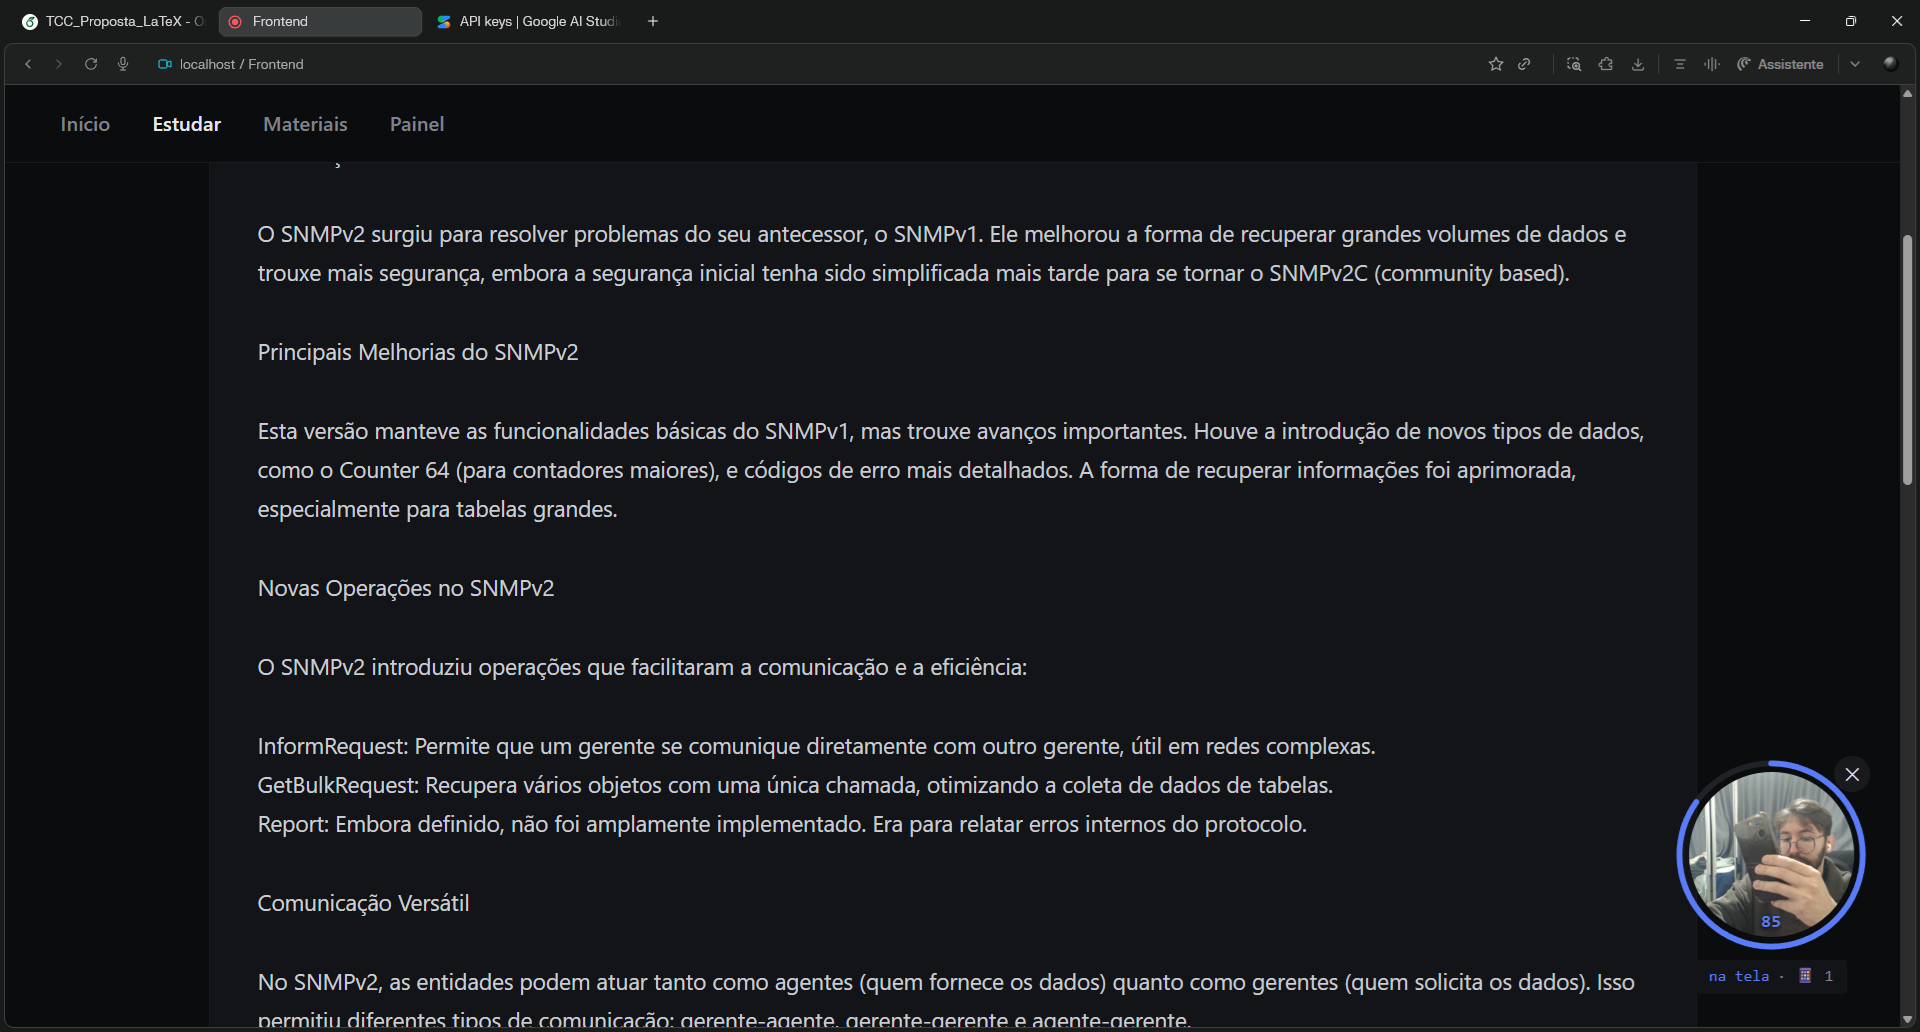
\includegraphics[width=0.48\textwidth]{foco-natela.png}\hfill
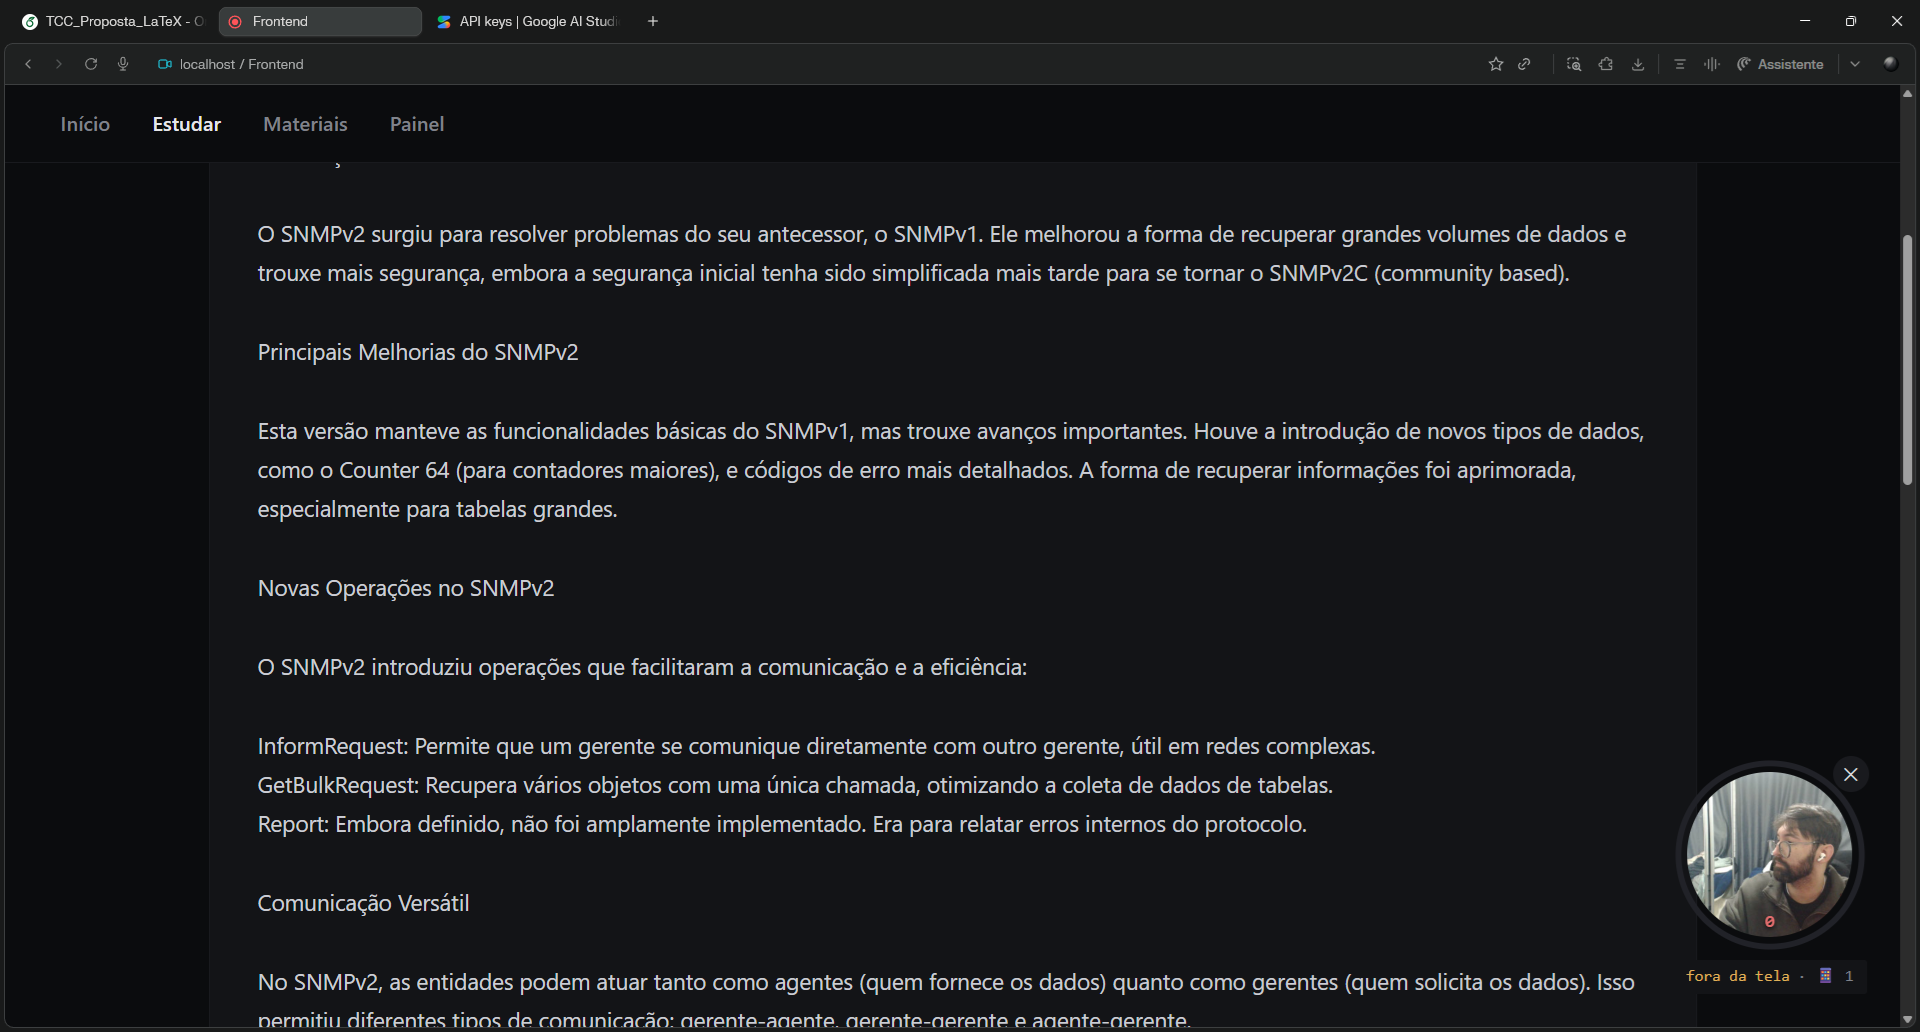
\includegraphics[width=0.48\textwidth]{foco-foratela.png}
\caption{Estados reconhecidos pelo monitoramento. À esquerda, rosto voltado para a tela, com um celular detectado no campo da câmera; à direita, olhar desviado da tela, com queda do \fs. Fonte: capturas do protótipo feitas pelo autor, com a própria imagem.}
\label{fig:foco-estados}
\end{figure}

\subsection{\label{sec:celular}Eventos de celular}

Em paralelo, a cada 1,2 s, o quadro atual é redimensionado para 640$\times$640 \estr{pixels}, com as bordas preenchidas para preservar a proporção, e submetido ao YOLOv8-nano pelo ONNX Runtime Web, em WebAssembly (WASM) com uma única \estr{thread}. Da saída da rede, o sistema extrai a maior pontuação atribuída à classe ``celular'' do COCO entre todas as posições candidatas, $c_j$. A inferência $j$ é positiva se $c_j > 0{,}35$. Um evento de celular é contado quando $k = 2$ inferências positivas consecutivas ocorrem, e um novo evento só pode começar depois que uma inferência negativa encerra o anterior. Com o intervalo de 1,2 s, isso significa que um celular precisa permanecer visível por cerca de 2,4 s para ser contado, o que filtra aparições acidentais. O número de eventos por intervalo de tempo é o segundo indicador enviado ao servidor.

\subsection{\label{sec:degradacao}Degradação graciosa}

Os dois modelos têm custos muito diferentes. A detecção facial é leve; o YOLO, mesmo na variante \estr{nano}, processa uma imagem de 640$\times$640 \estr{pixels} em uma rede convolucional, e seu tempo de inferência em WASM depende fortemente do processador. Em vez de exigir um computador mínimo, o \ferramenta degrada de forma graciosa: se o detector de celular não inicializa, ou se sua latência de inferência excede o intervalo de agendamento de 1,2 s de forma sustentada, ele é desligado, e a sessão continua apenas com o \fs. Se a própria detecção facial não inicializa, a sessão continua sem câmera, apenas com as questões. O modo de cada sessão (completo, sem celular ou sem câmera) é registrado junto com a telemetria. Essa decisão transforma uma limitação de \estr{hardware} em um comportamento previsível e mensurável, que é o objeto da QP2.

\section{\label{sec:mod3}Módulo 3: o painel de automonitoramento}

O painel (Figura~\ref{fig:painel}) devolve ao estudante, por disciplina, o tempo estudado, o tempo com \fs elevado, o \fs médio, o número de eventos de celular, o número de sessões e respostas, a taxa de acertos, a evolução do \fs minuto a minuto e a taxa de acertos por PDF. Seu propósito é alimentar o monitoramento do ciclo de autorregulação: tornar visível ao estudante, depois da sessão, o que ele não percebe durante ela.

\begin{figure}[htbp]
\centering
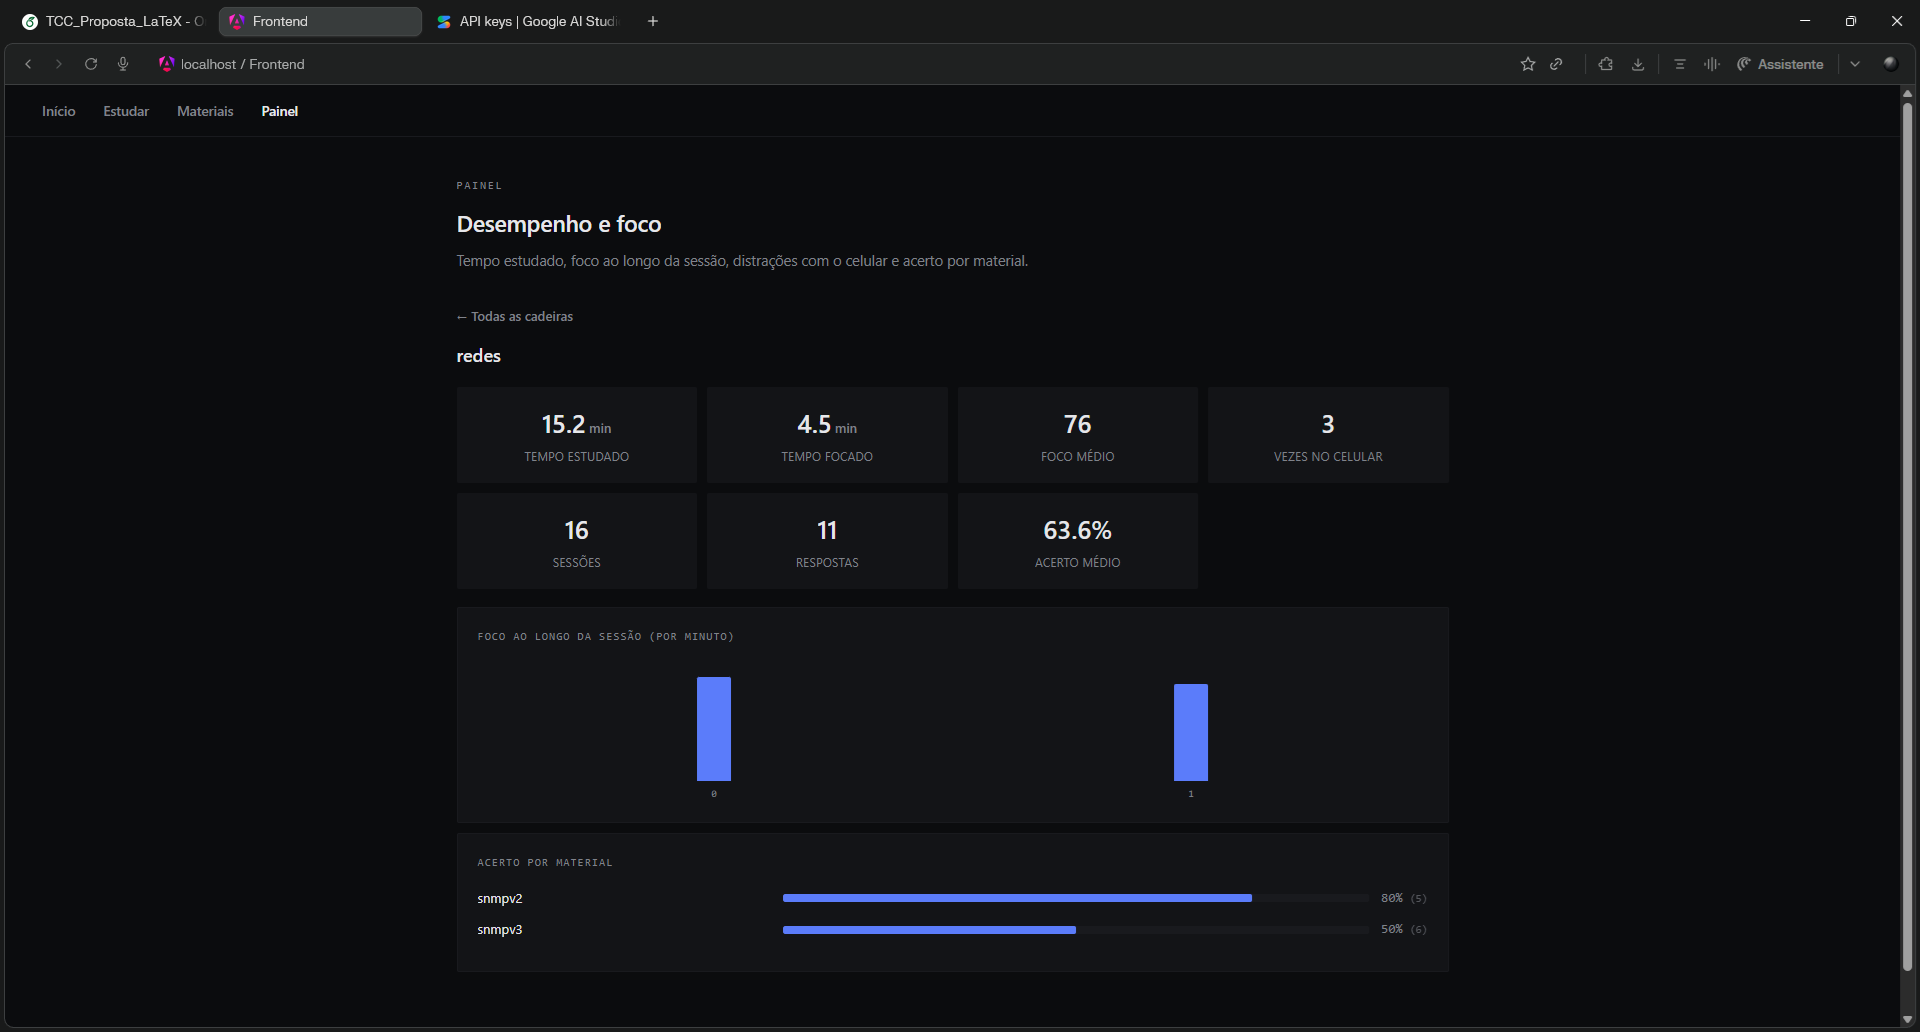
\includegraphics[width=0.85\textwidth]{painel.png}
\caption{Painel de automonitoramento de uma disciplina. Os valores exibidos provêm de sessões de teste do autor durante o desenvolvimento e ilustram apenas o \estr{layout}; não são resultados deste trabalho. Fonte: captura do protótipo feita pelo autor.}
\label{fig:painel}
\end{figure}

O painel cruza engajamento e desempenho, mas não afirma relação causal entre eles. Uma sessão com \fs baixo e muitos erros é um indício que o estudante pode interpretar, não um diagnóstico.

\section{\label{sec:fluxo}Fluxo de dados e privacidade}

O fluxo completo de uma sessão com câmera é o seguinte:
\begin{enumerate}
  \item O estudante envia o PDF; o servidor extrai, fragmenta e indexa o texto.
  \item O estudante inicia a sessão; o navegador carrega os modelos e calibra os limiares durante cinco segundos.
  \item A cada segundo, a interface atualiza o \fs exibido; a cada cinco segundos, grava uma amostra com o instante, o \fs, o número de novos eventos de celular e o modo da sessão; a cada quinze segundos, envia ao servidor o lote de amostras acumuladas.
  \item A cada questão, o fragmento-fonte correspondente foi enviado ao provedor do LLM no momento da geração, e a resposta do estudante é enviada ao servidor.
  \item O painel consulta o servidor, que agrega as amostras e as respostas.
\end{enumerate}

O fluxo tem duas fronteiras de privacidade distintas. A primeira, que envolve a imagem do estudante, é fechada por arquitetura: nenhum quadro de vídeo é serializado ou transmitido, e o servidor não tem sequer um \estr{endpoint} capaz de recebê-lo. A segunda, que envolve o texto do material, é aberta por necessidade: o fragmento-fonte precisa chegar ao modelo de linguagem, operado por terceiros. O estudante decide o que envia, mas deve ser informado de que o conteúdo dos PDFs sai do servidor da aplicação (Seção~\ref{sec:etica}). Há ainda um fluxo de dados de entrada menos evidente: os arquivos de execução e os pesos da detecção facial são baixados de redes de distribuição de conteúdo de terceiros, o que revela a esses serviços o endereço de rede do estudante, embora nenhuma imagem trafegue. A QP4 verifica a primeira fronteira e documenta os demais destinos contatados.

\section{\label{sec:parametros}Parâmetros da versão avaliada}

A Tabela~\ref{tab:parametros} reúne os parâmetros que definem o comportamento da versão avaliada. Os valores foram fixados antes da coleta e são os mesmos em todas as QPs, exceto nas análises de sensibilidade, que os variam de forma explícita.

\begin{table}[htbp]
\centering
\caption{Parâmetros da versão avaliada do \ferramenta. Fonte: código do protótipo \definir{versão/\estr{commit} congelado para a avaliação}.}
\label{tab:parametros}
\small
\begin{tabularx}{\textwidth}{>{\raggedright\arraybackslash}p{3.2cm} >{\raggedright\arraybackslash}X l}
\toprule
Componente & Parâmetro & Valor \\
\midrule
\multirow{3}{*}{Fragmentação} & Tamanho-alvo do fragmento & 900 caracteres \\
 & Sobreposição & 120 caracteres \\
 & Tamanho mínimo & 80 caracteres \\
\midrule
\multirow{2}{*}{Filtro de utilidade} & Mínimo de palavras & 15 \\
 & Máximo de palavras em caixa alta & 40\% \\
\midrule
\multirow{4}{*}{Geração} & Modelo de linguagem & \definir{modelo e versão} \\
 & Temperatura & 0,8 \\
 & Questões por chamada (lote) & 5 \\
 & \estr{Embeddings} & \definir{padrão do ChromaDB ou \estr{hashing}} \\
\midrule
\multirow{6}{*}{Engajamento visual} & Resolução de captura & 320$\times$240 \\
 & Duração da calibração & 5 s \\
 & Fator do limiar de EAR & 0,72 \\
 & Tolerâncias $\tau_y$, $\tau_p$ & 0,13; 0,10 \\
 & Período de tolerância $g$ & 2,5 s \\
 & Janela $\Delta$ & 8 s \\
\midrule
\multirow{4}{*}{Detecção de celular} & Entrada da rede & 640$\times$640 \\
 & Intervalo entre inferências & 1,2 s \\
 & Limiar de pontuação & 0,35 \\
 & Inferências consecutivas $k$ & 2 \\
\midrule
Telemetria & Amostragem / envio & 5 s / 15 s \\
\bottomrule
\end{tabularx}
\end{table}

Com o artefato definido, o próximo capítulo descreve como cada uma das promessas que ele assume será posta à prova.
